\documentclass{book}
\usepackage[pdftex]{graphicx} 
\usepackage{amsmath}
\usepackage{listings}

\begin{document}
\title{BEAST 2.0}
\maketitle

\section*{Vision}
To provide tools for computational science that are
\begin{itemize}
\item
1 {\em easy to use}, that is, well documented, have intuitive user interfaces with small learning curve.
\item
2 {\em open access}, that is, open source, open xml format, facilitating reproducability of results, runs
on many platforms.
\item
3 {\em easy to extend}, by having extensibility in design.
\end{itemize}

\section*{Scope}

Efficient Bayesian computation for sequence data analysis involving tree models.

\section*{Basic design}

Bayesian computation centers around MCMC algorithsm.
The basic structure of an MCMC algorithm is shown in Figure \ref{fig.mcmc}.
A glance at this bit of pseudo code reveals that the least that is required
are the following components:


\begin{figure}[h]
{\scriptsize
\begin{lstlisting}[frame=trbl]{}
Read data D
Initialize state S
L = likelihood(S, D)
while (not tired) {
    S' = proposed state
    L = likelihood(S', D)
    Accept or reject S'
    Log state
}
\end{lstlisting}
}
\caption{\label{fig.mcmc}Basic structur of MCMC.}
\end{figure}

\begin{itemize}
\item a data object that contains sequence data,
\item a state object to represent the current and proposed state.
The state consists of at least one tree (see scope) and parameters,
which are integer or real valued.
\item likelihood/density objects to calculate the posterior.
\item operator objects to work on the state and propose new states.
\item log objects, since we are interested in the results which have to be recorded
somewhere.
\item an MCMC object to control the flow of the computation.
\end{itemize}

So, that leaves us with at least a {\tt Data}, {\tt State}, {\tt Parameter}, 
{\tt Tree}, {\tt Likelihood}, {\tt Operator}, {\tt Log} and {\tt MCMC} object. Since trees
consist of nodes, a {\tt Node} object is desirable as well.

Since we want the system to be extensible (Vision 3), everything in the system is 
a {\tt Plugin} and can be replaced by a custom implementation. So, each of the above
objects are derived from {\tt Plugin}. To allow flexibility of plugins, every plugin 
can specify inputs. {\tt Input} objects contain information on type of the input and 
how they are stored in BEAST XML files.


\begin{figure}
\begin{center}
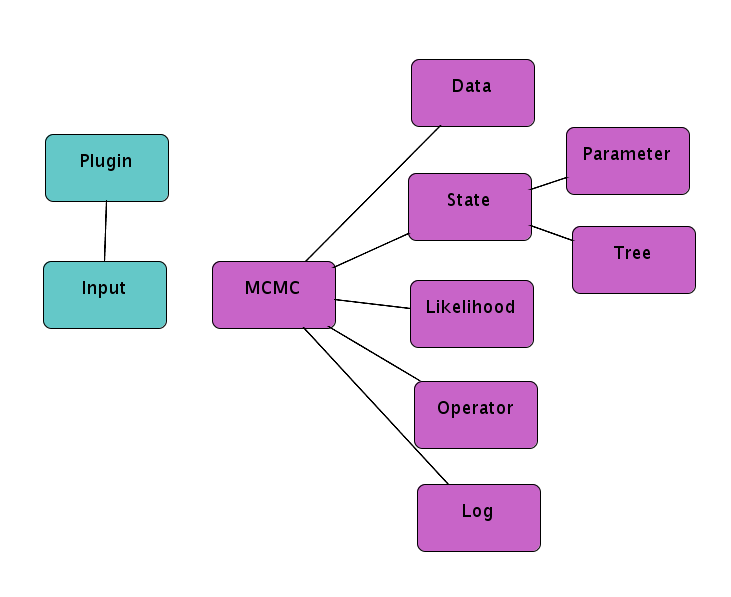
\includegraphics[width=10cm]{BEAST.png}
\end{center}
\caption{\label{fig.core}Core classes. Every class except {\tt Input} is derived
from {\tt Plugin}, but these relations are not shown in the diagram.}
\end{figure}






Basic structure of BEAST
- basic design

A closer look at the Core classes
- introducing interfaces for each of the classes
  - MCMC/Runable
  - Likelihood/Probability
  - Operator
  - Log
  - State
    - Tree
    - Parameter
  - Plugin
  - Input

BEAST 2.0 XML 
- file format and how the parser processing model
- Roll your own: extending through namespaces, maps

Nucleotide TreeLikelihood: an in depth look
- go in the gory details of TreeLikelihood, substitution models, etc

Recommended design patterns
- validation \& initialization patterns
- efficiency through store/restore





\end{document}

